\documentclass[11pt]{article}

\usepackage{amsmath}
\usepackage{amssymb}
\usepackage{fancyhdr}
\usepackage{comment}
\usepackage{color}
\usepackage{graphicx}
\usepackage[colorlinks=true,linkcolor=blue,urlcolor=blue]{hyperref}

\newcounter{marks}
\def\maxmarks#1{\extramark{#1}\addtocounter{marks}{#1}}
\def\extramark#1{
  \begin{flushright}
  [\emph{#1 points}]
  \end{flushright}
%  \quad\mbox{\LARGE\begin{tabular}{|c|c|}
%  \hline\rule{1cm}{0cm} & #1 \\ \hline \end{tabular}}
}
\def\dumptotal{%
\begin{flushright}
\begin{tabular}{|l|} \hline
\LARGE{\textbf{\rule{0pt}{16pt}Total:~\themarks}} \\ \hline
\end{tabular}
\end{flushright}}
\def\skiplines#1{\newline \forloop{#1}{{\rule{0pt}{20pt}} \\}}

\specialcomment{answer}{\color{blue}}{\color{black}}
\def\withanswers{\def\skiplines##1{\relax}\def\skippage{\relax}}
\def\withoutanswers{\excludecomment{answer}\def\skippage{\clearpage}}

\newif\ifprint
\printtrue

\oddsidemargin0cm
\topmargin-2cm     %I recommend adding these three lines to increase the
\textwidth16.5cm   %amount of usable space on the page (and save trees)
\textheight23.5cm

\newcommand{\mycoursenum}{10-601}
\newcommand{\myhwnum}{3}
\newcommand{\myname}{Jin Sun}
\newcommand{\myandrew}{your-andrew-id-here@andrew.cmu.edu}
\newcommand{\myfirstta}{Henry Gifford}
\newcommand{\mysecondta}{Jin Sun}

\newcommand{\question}[2] {\vspace{.25in} \hrule\vspace{0.5em} \noindent{\bf #1: #2} \vspace{0.5em} \hrule \vspace{.10in}}
\renewcommand{\part}[1] {\vspace{.10in} {\bf (#1)}}

\setlength{\parindent}{0pt}
\setlength{\parskip}{5pt plus 1pt}

\pagestyle{fancyplain}
\lhead{\fancyplain{}{\textbf{HW\myhwnum}}}
\ifprint
\rhead{\fancyplain{}{Andrew ID: \rule{0.2\textwidth}{.4pt}}}
\else
\rhead{\fancyplain{}{\myname\\ \myandrew}}
\fi
\chead{\fancyplain{}{\mycoursenum}}

\withoutanswers

\begin{document}

\medskip

\thispagestyle{plain}
\begin{center}
{\Large \mycoursenum: Homework \myhwnum} \\
Due: 9 October 2014 11:59pm (Autolab) \\
TAs: \myfirstta, \mysecondta \\
\medskip
\ifprint
Name: \rule{0.5\textwidth}{.4pt} \\
Andrew ID: \rule{0.45\textwidth}{.4pt} \\
\else
Name: \myname \\
Andrew ID: \myandrew \\
\fi
\end{center}

Please answer to the point, and do not spend time/space giving irrelevant details. You should not require more space than is provided for each question. If you do, please think whether you can make your argument more pithy, an exercise that can often lead to more insight into the problem. Please state any additional assumptions you make while answering the questions. You need to submit a single PDF file on autolab. Please make sure you write legibly for grading.

You can work in groups. However, no written notes can be shared, or taken during group discussions. You may ask clarifying questions on Piazza. However, under no circumstances should you reveal any part of the answer publicly on Piazza or any other public website. The intention of this policy is to facilitate learning, not circumvent it. Any incidents of plagiarism will be handled in accordance with \href{http://www.cmu.edu/policies/documents/Academic%20Integrity.htm}{CMU's Policy on Academic Integrity}.


%%%%%%%%%%%%%%%%%%%%%%%%%%%%%%%%%%%%%%%%%%%
\question{$\star$}{Code of Conduct Declaration}

\begin{itemize}
	\item Did you receive any help whatsoever from anyone in solving this assignment? Yes / No.
	\item If you answered \emph{yes}, give full details: \rule{0.4\textwidth}{.4pt} (e.g. \emph{Jane explained to me what is asked in Question 3.4})
	\item Did you give any help whatsoever to anyone in solving this assignment? Yes / No.
	\item If you answered \emph{yes}, give full details: \rule{0.4\textwidth}{.4pt} (e.g. \emph{I pointed Joe to section 2.3 to help him with Question 2}).
\end{itemize}

\question{$\star$}{Notifications}
This is the handout for theoretical questions in homework 3, you need to download the handout for programming part as well.
If you have any questions, please post it on Piazza or email:

\myfirstta: hgifford@andrew.cmu.edu

\mysecondta: jins@andrew.cmu.edu

%%%%%%%%%%%%%%%%%%%%%%%%%%%%%%%%%%%%%%%%%%%
\question{1}{Decision Boundaries and Complexity (TA:- \mysecondta)}
\part{a}
Figure \ref{db} in appendix shows three decision boundaries. Please list \textbf{all possible} decision boundaries for the following classifiers. Please write down the picture labels. No explanations required.

Decision Tree:

Logistic Regression for binary classification:

Perceptrons (Single-layer Neural Networks):

Multi-layer Neural Networks (Single Hidden Layer):
\maxmarks{8} \vspace*{0 cm}
\part{b}
For the four classifiers mentioned in part(a), analyse the separability and complexity on several datasets. For separability, you need to state whether the classifier is able to perfectly separate the data points. For complexity, you only need to state whether the decision tree need to be a full tree (at each leaf node there is no attribute to split) to achieve best performance. Please refer to the appendix for detailed explanation on these datasets.

\begin{itemize}
\item Logic OR
\item Logic XOR
\item Majority
\item Parity
\end{itemize}
\maxmarks{12} \vspace*{0 cm}
\question{2}{Activation Function (TA:- \mysecondta)}
In lectures we use the logistic sigmoid function as the activation function for logistic regression and neural networks. However, there are many other activation functions such as linear function, hyperbolic tangent function and Gaussian function. In this homework, you need to derive the gradient on \textbf{one sample} for logistic regression using hyperbolic tangent function as activation function.

The hyperbolic function is defined as follows:
\begin{equation}
\tanh(z)=\frac{\sinh(z)}{\cosh(z)}=\frac{e^z-e^{-z}}{e^z+e^{-z}}
\end{equation}

and you should calculate the following term:
\begin{equation}
\frac{\partial Loss(\textbf w)}{\partial (\textbf w)}
\end{equation}


Let's start with writing down the loss function on one sample for logistic regression:
\begin{equation}
Loss(\textbf{w})=-\ln P(Y=y|X=\textbf{x},\textbf{w})=-y\ln p-(1-y)\ln(1-p)
\end{equation}
where $p = \tanh(z)$ and $z = \textbf{w}^T\textbf{x}$

And then you should derive the derivative and use the chain rule to get the final answer.
\maxmarks{20} \vspace*{0 cm}

\dumptotal

\newpage
\question{3}{Appendix}
You do not need to include this page and the programming part into the pdf file for submission.

\begin{figure}[h]
    \centering
    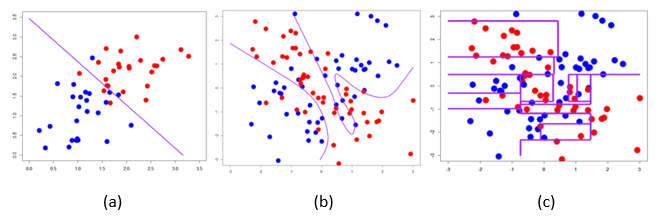
\includegraphics[scale=0.7]{figures/classifier.png}
    \caption{Decision Boundaries}
    \label{db}
\end{figure}

In the datasets for problem 1(b), each sample is a binary string contains zeros and ones, and each bit is a feature. The length of the strings are at least 2 and same among all samples.

\textbf{Logic OR}

The label of each string is the logic OR value among all the bits. For example, if $X_i$ is the $i$th digit in string $X$, the label is calculated by: $X_1$ OR $X_2$ OR $X_3 \hdots$

\textbf{Logic XOR}

The label of each string is the logic exclusive OR value among all the bits. For example, if $X_i$ is the $i$th digit in string $X$, the label is calculated by: $X_1$ XOR $X_2$ XOR $X_3 \hdots$

\textbf{Majority}

The label of each string is the digit with the most occurrence (either 0 or 1). The length of the strings is odd. For example, string ``$11110$'' has more 1s than 0s, so its label is 1.

\textbf{Parity}

If the string has odd number of zeros, the label will be 1; if the string has even number of zeros, the label will be 0. For example, string ``$101010$'' has 3 zeros, its label is 1.

\end{document}
